\chapter{Discount Factors and Forward Rate}\label{interpolation---practical-lesson-3}

In this chapter we will start to see the first applications of \texttt{python} to financial calculations.
In particular we will consider discount curves and forward rates, implementing the first utilities that will fill our financial module.
In addition we will briefly review a widely used mathematical tool: \emph{interpolation}.

\section{Linear interpolation}\label{linear-interpolation}

Interpolation is a method of constructing new points within the range of a discrete set of known data points.

Consider to have few data points, obtained by sampling or experimenting. These points represent the values of a function \(f(x)\), where \(x\) is an independent variable (e.g.~in recording a trip: distances at certain times, \(d = f(t)\)). It is often necessary to estimate the value of that function for intermediate values of the independent variable (e.g.~in our previous example what is the distance \(d\) at a new time \(t\) for which there isn't a sample ?).

\subsubsection{Example 1}\label{example-1}

Assume you are going on holidays by car and that luckily there isn't much traffic so that you can drive at constant speed (which gives a linear relation between travelled space and time i.e.~\(s = v \cdot t\), which means that if you plot the distances \(s\) as a function of the time \(t\) you get a line with slope \(v\)).

Given two samples of the car travelled distance \(s_1\) and \(s_2\) taken at two different times \(t_1\) and \(t_2\) you can linearly interpolate to find your position at different times using the following relations:

\[w = \frac{t - t_1}{t_2 - t_1}\]
where $t$ is a generic time at which we want to know the distance $s$)

\[s = (1 - w)\cdot s_1 + w \cdot s_2\]
where $s$ is the desired travelled distance.

\begin{tcolorbox}[breakable, size=fbox, boxrule=1pt, pad at break*=1mm,colback=cellbackground, colframe=cellborder]
\paragraph{Derivation:} the equation of a line for two points
\((t_1, s_1)\) and \((t_2, s_2)\) can be written as:

\[\frac{t - t_1}{t_2 - t_1} = \frac{s - s_1}{s_2 - s_1}\]

Setting \(w = \frac{t - t_1}{t_2 - t_1}\) and solving for \(s\) we find the desired solution:

\[w = \frac{t - t_1}{t_2 - t_1} \Rightarrow (s_2 - s_1)\cdot w = s - s_1 \Rightarrow ...\]
 \end{tcolorbox}
 
Back to our example, if
\(s_1 = 25.75~\mathrm{km}\;(@t_1 = 15~\mathrm{min})\) and
\(s_2 = 171.7~\mathrm{km}\;(@t_2 = 100~\mathrm{min})\) let's find distance travelled in 1 hour (interpolation):

\begin{tcolorbox}[breakable, size=fbox, boxrule=1pt, pad at break*=1mm,colback=cellbackground, colframe=cellborder]
\begin{Verbatim}[commandchars=\\\{\}]
\PY{n}{s\PYZus{}1} \PY{o}{=} \PY{l+m+mf}{25.75} \PY{c+c1}{\PYZsh{} distance in km}
\PY{n}{t\PYZus{}1} \PY{o}{=} \PY{l+m+mi}{15}    \PY{c+c1}{\PYZsh{} elapsed time in minutes}
\PY{n}{s\PYZus{}2} \PY{o}{=} \PY{l+m+mf}{171.7}
\PY{n}{t\PYZus{}2} \PY{o}{=} \PY{l+m+mi}{100}

\PY{n}{t} \PY{o}{=} \PY{l+m+mi}{60}

\PY{n}{w} \PY{o}{=} \PY{p}{(}\PY{n}{t} \PY{o}{\PYZhy{}} \PY{n}{t\PYZus{}1}\PY{p}{)}\PY{o}{/}\PY{p}{(}\PY{n}{t\PYZus{}2} \PY{o}{\PYZhy{}} \PY{n}{t\PYZus{}1}\PY{p}{)}
\PY{n}{s} \PY{o}{=} \PY{p}{(}\PY{l+m+mi}{1} \PY{o}{\PYZhy{}} \PY{n}{w}\PY{p}{)}\PY{o}{*}\PY{n}{s\PYZus{}1} \PY{o}{+} \PY{n}{w}\PY{o}{*}\PY{n}{s\PYZus{}2}

\PY{n+nb}{print} \PY{p}{(}\PY{l+s+s2}{\PYZdq{}}\PY{l+s+si}{\PYZob{}:.1f\PYZcb{}}\PY{l+s+s2}{ km}\PY{l+s+s2}{\PYZdq{}}\PY{o}{.}\PY{n}{format}\PY{p}{(}\PY{n}{s}\PY{p}{)}\PY{p}{)}

103.0 km
\end{Verbatim}
\end{tcolorbox}

Always interpret results with critically to understand if it makes sense or is wrong. In the previous example we certainly expected something between 25.75 and 171.7 km (our range ends) furthermore since we are looking for the distance at a time which is almost halfway the interval, the result will be somehow in the middle or around 98.6 km. This is indeed more or less what we have got.
This simple reasoning should be applied everytime you have a result to quickly judge it.

If we believe the relation between our variable stays the same, we can use the same formula to \emph{extrapolate} values \emph{outside} our initial sample. For example if we keep the same constant velocity in our trip we could check the distance travelled after 3 hours:

\begin{tcolorbox}[breakable, size=fbox, boxrule=1pt, pad at break*=1mm,colback=cellbackground, colframe=cellborder]
\begin{Verbatim}[commandchars=\\\{\}]
\PY{n}{s\PYZus{}1} \PY{o}{=} \PY{l+m+mf}{25.75} \PY{c+c1}{\PYZsh{} distance in km}
\PY{n}{t\PYZus{}1} \PY{o}{=} \PY{l+m+mi}{15}    \PY{c+c1}{\PYZsh{} elapsed time in minutes}
\PY{n}{s\PYZus{}2} \PY{o}{=} \PY{l+m+mf}{171.7}
\PY{n}{t\PYZus{}2} \PY{o}{=} \PY{l+m+mi}{100}

\PY{n}{t} \PY{o}{=} \PY{l+m+mi}{180}

\PY{n}{w} \PY{o}{=} \PY{p}{(}\PY{n}{t} \PY{o}{\PYZhy{}} \PY{n}{t\PYZus{}1}\PY{p}{)}\PY{o}{/}\PY{p}{(}\PY{n}{t\PYZus{}2} \PY{o}{\PYZhy{}} \PY{n}{t\PYZus{}1}\PY{p}{)}
\PY{n}{s} \PY{o}{=} \PY{p}{(}\PY{l+m+mi}{1} \PY{o}{\PYZhy{}} \PY{n}{w}\PY{p}{)}\PY{o}{*}\PY{n}{s\PYZus{}1} \PY{o}{+} \PY{n}{w}\PY{o}{*}\PY{n}{s\PYZus{}2}

\PY{n+nb}{print} \PY{p}{(}\PY{l+s+s2}{\PYZdq{}}\PY{l+s+si}{\PYZob{}:.1f\PYZcb{}}\PY{l+s+s2}{ km}\PY{l+s+s2}{\PYZdq{}}\PY{o}{.}\PY{n}{format}\PY{p}{(}\PY{n}{s}\PY{p}{)}\PY{p}{)}

309.1 km
\end{Verbatim}
\end{tcolorbox}

\subsection{Log-linear interpolation}\label{log-linear-interpolation}
When the variable we would like to interpolate has an exponential relation with the unknown we can fall back to the previous case by simply applying the logarithm on both sides of the relation. Doing so the previous formulas apply again except that at the end we have to exponentiate to get back the original variable. Assume the followign is the relationshipo between $p$ and $h$, two generic variables:

\[p = \mathrm{exp}(c \cdot h)\]

Applying the logarithm to both sides of the equation gives:

\[s = \mathrm{log}(p) = \mathrm{log}(\mathrm{exp}(c \cdot h)) = c \cdot h\]
which is a linear relation between the new variable $s$ and $h$. At this point we can use the results of the previous section to interpolate for values of the quantity $s$, just remeber to exponentiate the result to get the correct $p$. In formulas:

\[w = \frac{h - h_1}{h_2 - h_1}\]

\[s = (1 - w)\cdot s_1 + w \cdot s_2\;\;(\mathrm{remember \;now }\;s = \mathrm{log}(p))\]

\[p = \mathrm{exp}(s)\]

\subsubsection{Example 2}\label{example-2}

Atmospheric pressure decreases with the altitude (i.e.~the highest you flight the lower is the pressure) following an exponential law:

\[p = p_0\cdot e^{-\alpha h}\]
where
\begin{itemize}
\tightlist
\item
  \(h\) is the altitude
\item
  \(p_0\) is the pressure at sea level
\item
  \(\alpha\) is a constant
\end{itemize}

Taking the logarithm of each side of the equation I get a linear relation which can be interpolated as done before:

\[\tilde{s} = \mathrm{log}(p) = \mathrm{log}(p_0\cdot e^{-\alpha h})\propto - \alpha \cdot h\]

Now assume that we have measured
\(p_1 = 90~\mathrm{kPa}\;(h_1 = 1000~\mathrm{m})\) and
\(p_2 = 40~\mathrm{kPa}\;(h_1 = 7000~\mathrm{m})\) what will be the
atmospheric pressure on top of the Mont Blanc (\(4812~\mathrm{m}\)) ? and on top of Mount Everest (\(8848~\mathrm{m}\)) ?

\begin{tcolorbox}[breakable, size=fbox, boxrule=1pt, pad at break*=1mm,colback=cellbackground, colframe=cellborder]
\begin{Verbatim}[commandchars=\\\{\}]
\PY{c+c1}{\PYZsh{} pressure on top of the Mont Blanc (interpolation)}
\PY{k+kn}{from} \PY{n+nn}{math} \PY{k}{import} \PY{n}{log}\PY{p}{,} \PY{n}{exp}

\PY{c+c1}{\PYZsh{} first we take the logarithm of our measurements to use the linear }
\PY{c+c1}{\PYZsh{} relation to interpolate}
\PY{n}{h\PYZus{}1} \PY{o}{=} \PY{l+m+mi}{1000} \PY{c+c1}{\PYZsh{} height in meters}
\PY{n}{s\PYZus{}1} \PY{o}{=} \PY{n}{log}\PY{p}{(}\PY{l+m+mi}{90}\PY{p}{)} \PY{c+c1}{\PYZsh{} logarithm of the pressure at heigth h1}
\PY{n}{h\PYZus{}2} \PY{o}{=} \PY{l+m+mi}{7000} \PY{c+c1}{\PYZsh{} height in meters}
\PY{n}{s\PYZus{}2} \PY{o}{=} \PY{n}{log}\PY{p}{(}\PY{l+m+mi}{40}\PY{p}{)} \PY{c+c1}{\PYZsh{} logarithm of the pressure at heigth h2}

\PY{n}{h} \PY{o}{=} \PY{l+m+mi}{4812}

\PY{n}{w} \PY{o}{=} \PY{p}{(}\PY{n}{h} \PY{o}{\PYZhy{}} \PY{n}{h\PYZus{}1}\PY{p}{)}\PY{o}{/}\PY{p}{(}\PY{n}{h\PYZus{}2} \PY{o}{\PYZhy{}} \PY{n}{h\PYZus{}1}\PY{p}{)}
\PY{n}{s} \PY{o}{=} \PY{p}{(}\PY{l+m+mi}{1} \PY{o}{\PYZhy{}} \PY{n}{w}\PY{p}{)}\PY{o}{*}\PY{n}{s\PYZus{}1} \PY{o}{+} \PY{n}{w}\PY{o}{*}\PY{n}{s\PYZus{}2}

\PY{n+nb}{print} \PY{p}{(}\PY{l+s+s2}{\PYZdq{}}\PY{l+s+si}{\PYZob{}:.1f\PYZcb{}}\PY{l+s+s2}{ kPa}\PY{l+s+s2}{\PYZdq{}}\PY{o}{.}\PY{n}{format}\PY{p}{(}\PY{n}{exp}\PY{p}{(}\PY{n}{s}\PY{p}{)}\PY{p}{)}\PY{p}{)}

53.8 kPa
\end{Verbatim}
\end{tcolorbox}

\begin{tcolorbox}[breakable, size=fbox, boxrule=1pt, pad at break*=1mm,colback=cellbackground, colframe=cellborder]
\begin{Verbatim}[commandchars=\\\{\}]
\PY{c+c1}{\PYZsh{} pressure on top of the Mount Everest (extrapolation)}
\PY{k+kn}{from} \PY{n+nn}{math} \PY{k}{import} \PY{n}{log}\PY{p}{,} \PY{n}{exp}

\PY{c+c1}{\PYZsh{} first we take the logarithm of our measurements to use the linear }
\PY{c+c1}{\PYZsh{} relation to interpolate}
\PY{n}{h\PYZus{}1} \PY{o}{=} \PY{l+m+mi}{1000} \PY{c+c1}{\PYZsh{} height in meters}
\PY{n}{s\PYZus{}1} \PY{o}{=} \PY{n}{log}\PY{p}{(}\PY{l+m+mi}{90}\PY{p}{)} \PY{c+c1}{\PYZsh{} logarithm of the pressure at heigth h1}
\PY{n}{h\PYZus{}2} \PY{o}{=} \PY{l+m+mi}{7000} \PY{c+c1}{\PYZsh{} height in meters}
\PY{n}{s\PYZus{}2} \PY{o}{=} \PY{n}{log}\PY{p}{(}\PY{l+m+mi}{40}\PY{p}{)} \PY{c+c1}{\PYZsh{} logarithm of the pressure at heigth h2}

\PY{n}{h} \PY{o}{=} \PY{l+m+mi}{8848}

\PY{n}{w} \PY{o}{=} \PY{p}{(}\PY{n}{h} \PY{o}{\PYZhy{}} \PY{n}{h\PYZus{}1}\PY{p}{)}\PY{o}{/}\PY{p}{(}\PY{n}{h\PYZus{}2} \PY{o}{\PYZhy{}} \PY{n}{h\PYZus{}1}\PY{p}{)}
\PY{n}{s} \PY{o}{=} \PY{p}{(}\PY{l+m+mi}{1} \PY{o}{\PYZhy{}} \PY{n}{w}\PY{p}{)}\PY{o}{*}\PY{n}{s\PYZus{}1} \PY{o}{+} \PY{n}{w}\PY{o}{*}\PY{n}{s\PYZus{}2}

\PY{n+nb}{print} \PY{p}{(}\PY{l+s+s2}{\PYZdq{}}\PY{l+s+si}{\PYZob{}:.1f\PYZcb{}}\PY{l+s+s2}{ kPa}\PY{l+s+s2}{\PYZdq{}}\PY{o}{.}\PY{n}{format}\PY{p}{(}\PY{n}{exp}\PY{p}{(}\PY{n}{s}\PY{p}{)}\PY{p}{)}\PY{p}{)}

31.2 kPa
\end{Verbatim}
\end{tcolorbox}

\begin{figure}
\centering
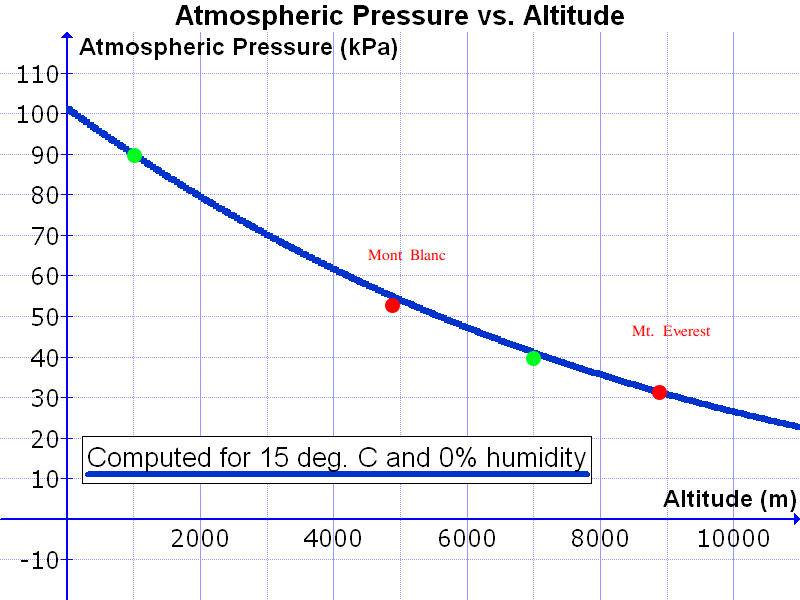
\includegraphics[width=0.6\linewidth]{Atmospheric_Pressure_vs._Altitude.png}
\caption{Atmospheric pressure versus altitude (wikipedia). Green points
represent our measurements, red points represent
interpolation/extrapolation.}
\end{figure}

\section{Discount curve interpolation}\label{discount-curve-interpolation}

Now we can come back to finance and using what we have just learnt try to write a function which interpolates some given discount factors.

Needed data:

\begin{itemize}
\tightlist
\item a list of pillars dates specifying the value dates of the given discount factors, \(t_0,...,t_{n-1}\);
\item a list of given discount factors, \(D(t_0),...,D(t_{n-1})\);
\item a pricing date (`today' date) which corresponds to \(t=0\).
\end{itemize}

The input argument to the function will be the value date at which we want to interpolate the discount factor. Since the discount factor can be expressed as \(D=e^{-r(T-t)}\) the function will use a log-linear interpolation to return the value at a date not included in the given pillars.

\[D(t) = \mathrm{exp}\Big( (1-w)\cdot \mathrm{ln}(D(t_i)) + w\cdot \mathrm{ln}(D(t_{i+1}))\Big);\;\;\;w=\frac{t-t_i}{t_{i+1}-t_i}\]
where \(i\) is such that \(t_i \le t \le t_{i+1}\). More technically we can say that we are doing a linear interpolation over time in the log space:

\[d(t_i):=\mathrm{ln}(D(t_i))\]

\[d(t) = (1-w)d(t_i) + wd(t_{i+1});\;\;\;w=\frac{t-t_i}{t_{i+1}-t_i}\]

\[D(t) = \mathrm{exp}(d(t))\]
where again \(i\) is such that \(t_i \le t \le t_{i+1}\)

Instead of reinventing the wheel and perform the interpolation with our own code, we'll use the function \texttt{interp} provided by the \texttt{python} module \texttt{numpy}; this function linearly interpolates the points to estimate the value of $f$ at some $x$.
Say we want to interpolate the points at $x = 2.5$ given the following values:

\begin{tcolorbox}[breakable, size=fbox, boxrule=1pt, pad at break*=1mm,colback=cellbackground, colframe=cellborder]
\begin{Verbatim}[commandchars=\\\{\}]
\PY{k+kn}{import} \PY{n+nn}{numpy} \PY{k}{as} \PY{n+nn}{np}

\PY{n}{xp} \PY{o}{=} \PY{p}{[}\PY{l+m+mi}{0}\PY{p}{,} \PY{l+m+mi}{1}\PY{p}{,} \PY{l+m+mi}{5}\PY{p}{]}
\PY{n}{fp} \PY{o}{=} \PY{p}{[}\PY{l+m+mi}{0}\PY{p}{,} \PY{l+m+mi}{2}\PY{p}{,} \PY{l+m+mi}{4}\PY{p}{]}
\PY{n}{np}\PY{o}{.}\PY{n}{interp}\PY{p}{(}\PY{l+m+mf}{2.5}\PY{p}{,} \PY{n}{xp}\PY{p}{,} \PY{n}{fp}\PY{p}{)}

2.75
\end{Verbatim}
\end{tcolorbox}

Assume we have three discount factors instead:
\begin{tcolorbox}[breakable, size=fbox, boxrule=1pt, pad at break*=1mm,colback=cellbackground, colframe=cellborder]
\begin{Verbatim}[commandchars=\\\{\}]
\PY{c+c1}{\PYZsh{} import modules and objects that we need}
\PY{k+kn}{from} \PY{n+nn}{datetime} \PY{k}{import} \PY{n}{date}
\PY{k+kn}{import} \PY{n+nn}{numpy}\PY{o}{,} \PY{n+nn}{math}
\PY{k+kn}{from} \PY{n+nn}{matplotlib} \PY{k}{import} \PY{n}{pyplot} \PY{k}{as} \PY{n}{plt}
\PY{k+kn}{import} \PY{n+nn}{matplotlib}\PY{n+nn}{.}\PY{n+nn}{dates} \PY{k}{as} \PY{n+nn}{mdates} 
\PY{c+c1}{\PYZsh{} with this notation we tell python to use mdates as an alias }
\PY{c+c1}{\PYZsh{} for matplotlib.dates}

\PY{c+c1}{\PYZsh{} define the input data}
\PY{n}{today\PYZus{}date} \PY{o}{=} \PY{n}{date}\PY{p}{(}\PY{l+m+mi}{2019}\PY{p}{,} \PY{l+m+mi}{10}\PY{p}{,} \PY{l+m+mi}{1}\PY{p}{)}

\PY{n}{pillar\PYZus{}dates} \PY{o}{=} \PY{p}{[}\PY{n}{date}\PY{p}{(}\PY{l+m+mi}{2019}\PY{p}{,} \PY{l+m+mi}{10}\PY{p}{,} \PY{l+m+mi}{1}\PY{p}{)}\PY{p}{,} \PY{n}{date}\PY{p}{(}\PY{l+m+mi}{2020}\PY{p}{,} \PY{l+m+mi}{10}\PY{p}{,} \PY{l+m+mi}{1}\PY{p}{)}\PY{p}{,} \PY{n}{date}\PY{p}{(}\PY{l+m+mi}{2021}\PY{p}{,} \PY{l+m+mi}{10}\PY{p}{,} \PY{l+m+mi}{1}\PY{p}{)}\PY{p}{]}
\PY{n}{discount\PYZus{}factors} \PY{o}{=} \PY{p}{[}\PY{l+m+mf}{1.0}\PY{p}{,} \PY{l+m+mf}{0.97}\PY{p}{,} \PY{l+m+mf}{0.72}\PY{p}{]}
\end{Verbatim}
\end{tcolorbox}
    
Let's see what this fake discount curve looks like when plotted on a graph:

\begin{tcolorbox}[breakable, size=fbox, boxrule=1pt, pad at break*=1mm,colback=cellbackground, colframe=cellborder]
\begin{Verbatim}[commandchars=\\\{\}]
\PY{n}{plt}\PY{o}{.}\PY{n}{plot}\PY{p}{(}\PY{n}{pillar\PYZus{}dates}\PY{p}{,} \PY{n}{discount\PYZus{}factors}\PY{p}{,} \PY{n}{marker}\PY{o}{=}\PY{l+s+s1}{\PYZsq{}}\PY{l+s+s1}{o}\PY{l+s+s1}{\PYZsq{}}\PY{p}{)}
\PY{n}{plt}\PY{o}{.}\PY{n}{gca}\PY{p}{(}\PY{p}{)}\PY{o}{.}\PY{n}{xaxis}\PY{o}{.}\PY{n}{set\PYZus{}major\PYZus{}formatter}\PY{p}{(}\PY{n}{mdates}\PY{o}{.}\PY{n}{DateFormatter}\PY{p}{(}\PY{l+s+s1}{\PYZsq{}}\PY{l+s+s1}{\PYZpc{}}\PY{l+s+s1}{m/}\PY{l+s+si}{\PYZpc{}d}\PY{l+s+s1}{/}\PY{l+s+s1}{\PYZpc{}}\PY{l+s+s1}{Y}\PY{l+s+s1}{\PYZsq{}}\PY{p}{)}\PY{p}{)}
\PY{n}{plt}\PY{o}{.}\PY{n}{gca}\PY{p}{(}\PY{p}{)}\PY{o}{.}\PY{n}{xaxis}\PY{o}{.}\PY{n}{set\PYZus{}major\PYZus{}locator}\PY{p}{(}\PY{n}{mdates}\PY{o}{.}\PY{n}{YearLocator}\PY{p}{(}\PY{p}{)}\PY{p}{)}
\PY{n}{plt}\PY{o}{.}\PY{n}{grid}\PY{p}{(}\PY{k+kc}{True}\PY{p}{)}
\PY{n}{plt}\PY{o}{.}\PY{n}{show}\PY{p}{(}\PY{p}{)}
\end{Verbatim}
\end{tcolorbox}

\begin{center}
\adjustimage{max size={0.9\linewidth}{0.9\paperheight}}{lecture_3_10_0.png}
\end{center}
{ \hspace*{\fill} \\}
    
Since it is a computation that from now on we need to perform quite often it is convenient to write a function that compute the discount factor at an arbitrary date.

\begin{tcolorbox}[breakable, size=fbox, boxrule=1pt, pad at break*=1mm,colback=cellbackground, colframe=cellborder]
\begin{Verbatim}[commandchars=\\\{\}]
\PY{c+c1}{\PYZsh{} define the df function}
\PY{k}{def} \PY{n+nf}{df}\PY{p}{(}\PY{n}{d}\PY{p}{)}\PY{p}{:}
    \PY{c+c1}{\PYZsh{} first thing we need to do is to apply the logarithm function}
    \PY{c+c1}{\PYZsh{} to the discount factors since we are doing log-linear and}
    \PY{c+c1}{\PYZsh{} not just linear interpolation}
    \PY{n}{log\PYZus{}discount\PYZus{}factors} \PY{o}{=} \PY{p}{[}\PY{p}{]}
    \PY{k}{for} \PY{n}{discount\PYZus{}factor} \PY{o+ow}{in} \PY{n}{discount\PYZus{}factors}\PY{p}{:}
        \PY{n}{log\PYZus{}discount\PYZus{}factors}\PY{o}{.}\PY{n}{append}\PY{p}{(}\PY{n}{math}\PY{o}{.}\PY{n}{log}\PY{p}{(}\PY{n}{discount\PYZus{}factor}\PY{p}{)}\PY{p}{)}
    
    \PY{c+c1}{\PYZsh{} perform the linear interpolation of the log discount factors}
    \PY{n}{interpolated\PYZus{}log\PYZus{}discount\PYZus{}factor} \PY{o}{=} \PYZbs{}
        \PY{n}{numpy}\PY{o}{.}\PY{n}{interp}\PY{p}{(}\PY{n}{d}\PY{p}{,} \PY{n}{pillar\PYZus{}dates}\PY{p}{,} \PY{n}{log\PYZus{}discount\PYZus{}factors}\PY{p}{)}
    
    \PY{c+c1}{\PYZsh{} return the interpolated discount factor}
    \PY{k}{return} \PY{n}{math}\PY{o}{.}\PY{n}{exp}\PY{p}{(}\PY{n}{interpolated\PYZus{}log\PYZus{}discount\PYZus{}factor}\PY{p}{)}
\end{Verbatim}
\end{tcolorbox}

This is almost OK, \textbf{but it won't work} because \texttt{numpy.interp} only accepts numbers/lists of numbers as arguments i.e.~it doesn't automatically convert or interpret dates as numbers and doesn't know how to interpolate them. So we need to do the conversion ourselves before passing the dates into the interpolation function.
The following updated version of our function converts the pillar dates into ``pillar days'' i.e. each date is replaced by the number of days today ($t_0$):

\begin{tcolorbox}[breakable, size=fbox, boxrule=1pt, pad at break*=1mm,colback=cellbackground, colframe=cellborder]
\begin{Verbatim}[commandchars=\\\{\}]
\PY{k}{def} \PY{n+nf}{df}\PY{p}{(}\PY{n}{d}\PY{p}{)}\PY{p}{:}
    \PY{c+c1}{\PYZsh{} first thing we need to do is to apply the logarithm function}
    \PY{c+c1}{\PYZsh{} to the discount factors since we are doing log-linear and}
    \PY{c+c1}{\PYZsh{} not just linear interpolation}
    \PY{n}{log\PYZus{}discount\PYZus{}factors} \PY{o}{=} \PY{p}{[}\PY{p}{]}
    \PY{k}{for} \PY{n}{discount\PYZus{}factor} \PY{o+ow}{in} \PY{n}{discount\PYZus{}factors}\PY{p}{:}
        \PY{n}{log\PYZus{}discount\PYZus{}factors}\PY{o}{.}\PY{n}{append}\PY{p}{(}\PY{n}{math}\PY{o}{.}\PY{n}{log}\PY{p}{(}\PY{n}{discount\PYZus{}factor}\PY{p}{)}\PY{p}{)}
    
    \PY{c+c1}{\PYZsh{} convert the pillar dates to pillar \PYZsq{}days\PYZsq{}}
    \PY{c+c1}{\PYZsh{} i.e. number of days from today}
    \PY{c+c1}{\PYZsh{} to write shorter code we can use this NEW notation}
    \PY{c+c1}{\PYZsh{} which condenses for and list creation in one line}
    \PY{n}{pillar\PYZus{}days} \PY{o}{=} \PYZbs{}
        \PY{p}{[}\PY{p}{(}\PY{n}{pillar\PYZus{}date} \PY{o}{\PYZhy{}} \PY{n}{today\PYZus{}date}\PY{p}{)}\PY{o}{.}\PY{n}{days} \PY{k}{for} \PY{n}{pillar\PYZus{}date} \PY{o+ow}{in} \PY{n}{pillar\PYZus{}dates}\PY{p}{]}
    
    \PY{c+c1}{\PYZsh{} obviously we need to do the same to the value date}
    \PY{c+c1}{\PYZsh{} argument of the df function}
    \PY{n}{d\PYZus{}days} \PY{o}{=} \PY{p}{(}\PY{n}{d} \PY{o}{\PYZhy{}} \PY{n}{today\PYZus{}date}\PY{p}{)}\PY{o}{.}\PY{n}{days}
    
    \PY{c+c1}{\PYZsh{} perform the linear interpolation of the log discount factors}
    \PY{n}{interpolated\PYZus{}log\PYZus{}discount\PYZus{}factor} \PY{o}{=} \PYZbs{}
        \PY{n}{numpy}\PY{o}{.}\PY{n}{interp}\PY{p}{(}\PY{n}{d\PYZus{}days}\PY{p}{,} \PY{n}{pillar\PYZus{}days}\PY{p}{,} \PY{n}{log\PYZus{}discount\PYZus{}factors}\PY{p}{)}
    
    \PY{c+c1}{\PYZsh{} return the interpolated discount factor}
    \PY{k}{return} \PY{n}{math}\PY{o}{.}\PY{n}{exp}\PY{p}{(}\PY{n}{interpolated\PYZus{}log\PYZus{}discount\PYZus{}factor}\PY{p}{)}
\end{Verbatim}
\end{tcolorbox}

Now we can use the \texttt{df} function to get discount factors on value dates between the given pillar dates:

\begin{tcolorbox}[breakable, size=fbox, boxrule=1pt, pad at break*=1mm,colback=cellbackground, colframe=cellborder]
\begin{Verbatim}[commandchars=\\\{\}]
\PY{n}{d0} \PY{o}{=} \PY{n}{date}\PY{p}{(}\PY{l+m+mi}{2020}\PY{p}{,} \PY{l+m+mi}{1}\PY{p}{,} \PY{l+m+mi}{1}\PY{p}{)}
\PY{n}{df0} \PY{o}{=} \PY{n}{df}\PY{p}{(}\PY{n}{d0}\PY{p}{)}
\PY{n+nb}{print} \PY{p}{(}\PY{n}{df0}\PY{p}{)}

0.9923728228571693
\end{Verbatim}
\end{tcolorbox}

\begin{tcolorbox}[breakable, size=fbox, boxrule=1pt, pad at break*=1mm,colback=cellbackground, colframe=cellborder]
\begin{Verbatim}[commandchars=\\\{\}]
\PY{n}{d1} \PY{o}{=} \PY{n}{date}\PY{p}{(}\PY{l+m+mi}{2021}\PY{p}{,} \PY{l+m+mi}{1}\PY{p}{,} \PY{l+m+mi}{1}\PY{p}{)}
\PY{n}{df1} \PY{o}{=} \PY{n}{df}\PY{p}{(}\PY{n}{d1}\PY{p}{)}
\PY{n+nb}{print} \PY{p}{(}\PY{n}{df1}\PY{p}{)}

0.8997999273630835
\end{Verbatim}
\end{tcolorbox}

Another very useful way to check the correctness of a result is by plotting data, so let's see what these look like when plotted on a semi-log graph and if they make sense:
    
\begin{tcolorbox}[breakable, size=fbox, boxrule=1pt, pad at break*=1mm,colback=cellbackground, colframe=cellborder]
\begin{Verbatim}[commandchars=\\\{\}]
\PY{k+kn}{from} \PY{n+nn}{matplotlib} \PY{k}{import} \PY{n}{pyplot} \PY{k}{as} \PY{n}{plt}
\PY{k+kn}{import} \PY{n+nn}{matplotlib}\PY{n+nn}{.}\PY{n+nn}{dates} \PY{k}{as} \PY{n+nn}{mdates}

\PY{n}{plt}\PY{o}{.}\PY{n}{semilogy}\PY{p}{(}\PY{n}{pillar\PYZus{}dates}\PY{p}{,} \PY{n}{discount\PYZus{}factors}\PY{p}{,} \PY{n}{marker}\PY{o}{=}\PY{l+s+s1}{\PYZsq{}}\PY{l+s+s1}{o}\PY{l+s+s1}{\PYZsq{}}\PY{p}{)}
\PY{n}{plt}\PY{o}{.}\PY{n}{semilogy}\PY{p}{(}\PY{n}{d0}\PY{p}{,}\PY{n}{df0} \PY{p}{,} \PY{n}{marker}\PY{o}{=}\PY{l+s+s1}{\PYZsq{}}\PY{l+s+s1}{X}\PY{l+s+s1}{\PYZsq{}}\PY{p}{)}
\PY{n}{plt}\PY{o}{.}\PY{n}{semilogy}\PY{p}{(}\PY{n}{d1}\PY{p}{,}\PY{n}{df1} \PY{p}{,} \PY{n}{marker}\PY{o}{=}\PY{l+s+s1}{\PYZsq{}}\PY{l+s+s1}{X}\PY{l+s+s1}{\PYZsq{}}\PY{p}{)}
\PY{n}{plt}\PY{o}{.}\PY{n}{gca}\PY{p}{(}\PY{p}{)}\PY{o}{.}\PY{n}{xaxis}\PY{o}{.}\PY{n}{set\PYZus{}major\PYZus{}formatter}\PY{p}{(}\PY{n}{mdates}\PY{o}{.}\PY{n}{DateFormatter}\PY{p}{(}\PY{l+s+s1}{\PYZsq{}}\PY{l+s+s1}{\PYZpc{}}\PY{l+s+s1}{m/}\PY{l+s+si}{\PYZpc{}d}\PY{l+s+s1}{/}\PY{l+s+s1}{\PYZpc{}}\PY{l+s+s1}{Y}\PY{l+s+s1}{\PYZsq{}}\PY{p}{)}\PY{p}{)}
\PY{n}{plt}\PY{o}{.}\PY{n}{gca}\PY{p}{(}\PY{p}{)}\PY{o}{.}\PY{n}{xaxis}\PY{o}{.}\PY{n}{set\PYZus{}major\PYZus{}locator}\PY{p}{(}\PY{n}{mdates}\PY{o}{.}\PY{n}{YearLocator}\PY{p}{(}\PY{p}{)}\PY{p}{)}
\PY{n}{plt}\PY{o}{.}\PY{n}{grid}\PY{p}{(}\PY{k+kc}{True}\PY{p}{)}
\PY{n}{plt}\PY{o}{.}\PY{n}{show}\PY{p}{(}\PY{p}{)}
\end{Verbatim}
\end{tcolorbox}

\begin{center}
\adjustimage{max size={0.9\linewidth}{0.9\paperheight}}{lecture_3_15_0.png}
\end{center}
    { \hspace*{\fill} \\}

Let's see what these look like when plotted on a linear graph instead:
    
\begin{tcolorbox}[breakable, size=fbox, boxrule=1pt, pad at break*=1mm,colback=cellbackground, colframe=cellborder]
\begin{Verbatim}[commandchars=\\\{\}]
\PY{k+kn}{from} \PY{n+nn}{matplotlib} \PY{k}{import} \PY{n}{pyplot} \PY{k}{as} \PY{n}{plt}
\PY{k+kn}{import} \PY{n+nn}{matplotlib}\PY{n+nn}{.}\PY{n+nn}{dates} \PY{k}{as} \PY{n+nn}{mdates}
\PY{n}{plt}\PY{o}{.}\PY{n}{plot}\PY{p}{(}\PY{n}{pillar\PYZus{}dates}\PY{p}{,} \PY{n}{discount\PYZus{}factors}\PY{p}{,} \PY{n}{marker}\PY{o}{=}\PY{l+s+s1}{\PYZsq{}}\PY{l+s+s1}{o}\PY{l+s+s1}{\PYZsq{}}\PY{p}{)}
\PY{n}{plt}\PY{o}{.}\PY{n}{plot}\PY{p}{(}\PY{n}{d0}\PY{p}{,}\PY{n}{df0} \PY{p}{,} \PY{n}{marker}\PY{o}{=}\PY{l+s+s1}{\PYZsq{}}\PY{l+s+s1}{X}\PY{l+s+s1}{\PYZsq{}}\PY{p}{)}
\PY{n}{plt}\PY{o}{.}\PY{n}{plot}\PY{p}{(}\PY{n}{d1}\PY{p}{,}\PY{n}{df1} \PY{p}{,} \PY{n}{marker}\PY{o}{=}\PY{l+s+s1}{\PYZsq{}}\PY{l+s+s1}{X}\PY{l+s+s1}{\PYZsq{}}\PY{p}{)}
\PY{n}{plt}\PY{o}{.}\PY{n}{gca}\PY{p}{(}\PY{p}{)}\PY{o}{.}\PY{n}{xaxis}\PY{o}{.}\PY{n}{set\PYZus{}major\PYZus{}formatter}\PY{p}{(}\PY{n}{mdates}\PY{o}{.}\PY{n}{DateFormatter}\PY{p}{(}\PY{l+s+s1}{\PYZsq{}}\PY{l+s+s1}{\PYZpc{}}\PY{l+s+s1}{m/}\PY{l+s+si}{\PYZpc{}d}\PY{l+s+s1}{/}\PY{l+s+s1}{\PYZpc{}}\PY{l+s+s1}{Y}\PY{l+s+s1}{\PYZsq{}}\PY{p}{)}\PY{p}{)}
\PY{n}{plt}\PY{o}{.}\PY{n}{gca}\PY{p}{(}\PY{p}{)}\PY{o}{.}\PY{n}{xaxis}\PY{o}{.}\PY{n}{set\PYZus{}major\PYZus{}locator}\PY{p}{(}\PY{n}{mdates}\PY{o}{.}\PY{n}{YearLocator}\PY{p}{(}\PY{p}{)}\PY{p}{)}
\PY{n}{plt}\PY{o}{.}\PY{n}{grid}\PY{p}{(}\PY{k+kc}{True}\PY{p}{)}
\PY{n}{plt}\PY{o}{.}\PY{n}{show}\PY{p}{(}\PY{p}{)}
\end{Verbatim}
\end{tcolorbox}

\begin{center}
\adjustimage{max size={0.9\linewidth}{0.9\paperheight}}{lecture_3_16_0.png}
\end{center}
    { \hspace*{\fill} \\}

\section{Calculating Forward Rates}\label{calculating-forward-rates}

A forward rate is an interest rate applicable to a financial transaction that will take place in the future. Forward rates are calculated from the spot rate and by exploiting no arbitrage condition i.e investing at rate \(r_1\) for the period \((0, T_1)\) and then \emph{reinvesting} at rate \(r_{1,2}\) for the time period \((T_1, T_2)\) is equivalent to invest at rate \(r_2\) for the full time period \((0, T_2)\) (two investors shouldn't be able to earn money from arbitraging between different interest periods). That said:

\[(1+r_1 T_1)(1+r_{1,2}(T_2 - T_1)) = 1 + r_2 T_2\]

Solving for \(r_{1,2}\) leads to

\[F(T_1, T_2) = r_{1,2} = \frac{1}{T_2-T_1}\Big(\frac{D(T_1)}{D(T_2)} - 1 \Big)~~~~\textrm{(where $D{(T_i)}=\frac{1}{1+r_iT_{i}}$)}\]

\begin{tcolorbox}[breakable, size=fbox, boxrule=1pt, pad at break*=1mm,colback=cellbackground, colframe=cellborder]
\begin{Verbatim}[commandchars=\\\{\}]
\PY{k+kn}{from} \PY{n+nn}{datetime} \PY{k}{import} \PY{n}{date}
\PY{k+kn}{import} \PY{n+nn}{numpy}\PY{o}{,} \PY{n+nn}{math}

\PY{n}{today\PYZus{}date} \PY{o}{=} \PY{n}{date} \PY{p}{(}\PY{l+m+mi}{2019}\PY{p}{,} \PY{l+m+mi}{1}\PY{p}{,} \PY{l+m+mi}{1}\PY{p}{)}

\PY{n}{pillar\PYZus{}dates} \PY{o}{=} \PY{p}{[}\PY{n}{date}\PY{p}{(}\PY{l+m+mi}{2019} \PY{p}{,} \PY{l+m+mi}{1} \PY{p}{,}\PY{l+m+mi}{1}\PY{p}{)}\PY{p}{,} 
                \PY{n}{date}\PY{p}{(}\PY{l+m+mi}{2020}\PY{p}{,} \PY{l+m+mi}{1}\PY{p}{,} \PY{l+m+mi}{1}\PY{p}{)}\PY{p}{,} 
                \PY{n}{date}\PY{p}{(}\PY{l+m+mi}{2021}\PY{p}{,} \PY{l+m+mi}{10} \PY{p}{,}\PY{l+m+mi}{1}\PY{p}{)}\PY{p}{]}
\PY{n}{discount\PYZus{}factors} \PY{o}{=} \PY{p}{[}\PY{l+m+mf}{1.0}\PY{p}{,} \PY{l+m+mf}{0.97}\PY{p}{,} \PY{l+m+mf}{0.72}\PY{p}{]}

\PY{k}{def} \PY{n+nf}{forward\PYZus{}rate}\PY{p}{(}\PY{n}{t1}\PY{p}{,} \PY{n}{t2}\PY{p}{)}\PY{p}{:}
    \PY{k}{return} \PY{l+m+mf}{365.0}\PY{o}{/}\PY{p}{(}\PY{n}{t2}\PY{o}{\PYZhy{}}\PY{n}{t1}\PY{p}{)}\PY{o}{.}\PY{n}{days} \PY{o}{*} \PY{p}{(}\PY{n}{df}\PY{p}{(}\PY{n}{t1}\PY{p}{)} \PY{o}{/} \PY{n}{df}\PY{p}{(}\PY{n}{t2}\PY{p}{)} \PY{o}{\PYZhy{}} \PY{l+m+mi}{1}\PY{p}{)}

\PY{n}{forward\PYZus{}rate}\PY{p}{(}\PY{n}{date}\PY{p}{(}\PY{l+m+mi}{2019}\PY{p}{,} \PY{l+m+mi}{2}\PY{p}{,} \PY{l+m+mi}{1}\PY{p}{)}\PY{p}{,} \PY{n}{date}\PY{p}{(}\PY{l+m+mi}{2019}\PY{p}{,} \PY{l+m+mi}{8}\PY{p}{,} \PY{l+m+mi}{1}\PY{p}{)}\PY{p}{)}
\end{Verbatim}
\end{tcolorbox}

\subsection{2008 Financial Crisis}\label{financial-crisis}

Looking at the historical series of the Euribor (6M) rate versus the Eonia Overnight Indexed Swap (OIS-6M) rate over the time interval 2006-2011 it becomes apparent how before August 2007 the two rates display strictly overlapping trends differing of no more than 6 bps.

\begin{figure}[h]
\centering
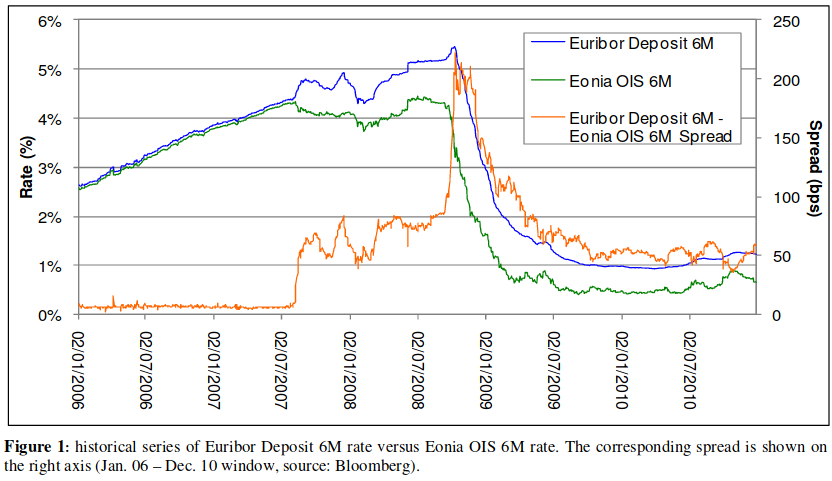
\includegraphics[width=0.7\linewidth]{credit_crunch.png}
\end{figure}

In August 2007 however we observe a sudden increase of the Euribor rate and a simultaneous decrease of the OIS rate that leads to the explosion of the corresponding basis spread, touching the peak of 222 bps in October 2008, when Lehman Brothers filed for bankruptcy. Successively the basis has sensibly reduced and stabilized between 40 bps and 60 bps (notice that the pre-crisis level has never been recovered). The same effect is observed for other similar couples of series, e.g.~Euribor 3M vs OIS 3M.

The reason of the abrupt divergence between the Euribor and OIS rates can be explained by considering both the monetary policy decisions adopted by international authorities in response to the financial turmoil, and the impact of the credit crunch on the credit and liquidity risk perception of the market, coupled with the different financial meaning and dynamics of these rates.

\begin{itemize}
\tightlist
\item
  The Euribor rate is the reference rate for over-the-counter (OTC)
  transactions in the Euro area. It is defined as \underline{the rate at which
  Euro interbank Deposits are being offered within the EMU zone by one
  prime bank to another at 11:00 a.m. Brussels time}. The rate fixings
  for a strip of 15 maturities (from one day to one year) are
  constructed as the average of the rates submitted (excluding the
  highest and lowest 15\% tails) by a panel of 42 banks, selected
  among the EU banks with the highest volume of business in the Euro
  zone money markets, plus some large international bank from non-EU
  countries with important euro zone operations. \textbf{Thus, Euribor
  rates reflect the average cost of funding of banks in the interbank
  market at each given maturity. During the crisis the solvency and
  solidity of the whole financial sector was brought into question and
  the credit and liquidity risk and premia associated to interbank
  counterparties sharply increased.} The Euribor rates immediately
  reflected these dynamics and raise to their highest values over more
  than 10 years. As seen in the plot above, the Euribor 6M rate suddenly
  increased on August 2007 and reached 5.49\% on 10th October 2008.
\item
  The Eonia rate is the reference rate for overnight OTC transactions in
  the Euro area. It is constructed as \underline{the average rate of the overnight
  transactions (one day maturity deposits) executed during a given
  business day} by a panel of banks on the interbank money market,
  weighted with the corresponding transaction volumes. \textbf{The Eonia
  Contribution Panel coincides with the Euribor Contribution Panel, thus
  Eonia rate includes information on the short term (overnight)
  liquidity expectations of banks in the Euro money market. It is also
  used by the European Central Bank (ECB) as a method of effecting and
  observing the transmission of its monetary policy actions. During the
  crisis the central banks were mainly concerned about restabilising the
  level of liquidity in the market, thus they reduced the level of the
  official rates.} Furthermore, the daily tenor of the Eonia rate makes
  negligible the credit and liquidity risks reflected on it: for this
  reason the OIS rates are considered the best proxies available in the
  market for the risk-free rate.
\end{itemize}

As a practial result of the divergence of the two indices, after the 2008 financial crisis, it is not possible anymore to use a single discount curve to correctly price forward rates of all tenors. For example, if we want to calculate the net present value of a forward 6-month libor coupon, we need to simultaneously use two different discount curves:

\begin{itemize}
\tightlist
\item the 6-month libor curve for determining the forward rate;
\item the EONIA curve for discounting the expected cash flow.
\end{itemize}

We are now going to explore how to implement the following calculation:

\[\mathrm{NPV} = D_{\mathrm{EONIA}}(T_1) \times \frac{1}{T_2-T_1}\Big(\frac{D_{\mathrm{LIBOR}}(T_1)}{D_{\mathrm{LIBOR}}(T_2)} - 1 \Big)\]

Every object oriented language allows for a design pattern, that uses containers (in \texttt{python} dictionaries) to group together data, then having functions operate on those containers (or dictionaries), perhaps with a few additional parameters. This is easily doable with \textbf{classes}.

Now we can finally write a \texttt{DiscountCurve} class which contains the pillar dates and pillar discount factors as attributes and which has methods for calculating the discount factor and forward rate at arbitrary dates.

\begin{tcolorbox}[breakable, size=fbox, boxrule=1pt, pad at break*=1mm,colback=cellbackground, colframe=cellborder]
\begin{Verbatim}[commandchars=\\\{\}]
\PY{k+kn}{import} \PY{n+nn}{math}
\PY{k+kn}{import} \PY{n+nn}{numpy}
\PY{k+kn}{from} \PY{n+nn}{datetime} \PY{k}{import} \PY{n}{date}

\PY{k}{class} \PY{n+nc}{DiscountCurve}\PY{p}{:}

    \PY{k}{def} \PY{n+nf}{\PYZus{}\PYZus{}init\PYZus{}\PYZus{}}\PY{p}{(}\PY{n+nb+bp}{self}\PY{p}{,} \PY{n}{today}\PY{p}{,} \PY{n}{pillar\PYZus{}dates}\PY{p}{,} \PY{n}{discount\PYZus{}factors}\PY{p}{)}\PY{p}{:}
        \PY{n+nb+bp}{self}\PY{o}{.}\PY{n}{today} \PY{o}{=} \PY{n}{today}
        \PY{n+nb+bp}{self}\PY{o}{.}\PY{n}{pillar\PYZus{}dates} \PY{o}{=} \PY{n}{pillar\PYZus{}dates}
        \PY{n+nb+bp}{self}\PY{o}{.}\PY{n}{discount\PYZus{}factors} \PY{o}{=} \PY{n}{discount\PYZus{}factors}

    \PY{k}{def} \PY{n+nf}{df}\PY{p}{(}\PY{n+nb+bp}{self}\PY{p}{,} \PY{n}{d}\PY{p}{)}\PY{p}{:}
        \PY{n}{log\PYZus{}discount\PYZus{}factors} \PY{o}{=} \PYZbs{}
          \PY{p}{[}\PY{n}{math}\PY{o}{.}\PY{n}{log}\PY{p}{(}\PY{n}{discount\PYZus{}factor}\PY{p}{)} 
           \PY{k}{for} \PY{n}{discount\PYZus{}factor} \PY{o+ow}{in} \PY{n+nb+bp}{self}\PY{o}{.}\PY{n}{discount\PYZus{}factors}\PY{p}{]}
        \PY{n}{pillar\PYZus{}days} \PY{o}{=} \PY{p}{[}\PY{p}{(}\PY{n}{pillar\PYZus{}date} \PY{o}{\PYZhy{}} \PY{n+nb+bp}{self}\PY{o}{.}\PY{n}{today}\PY{p}{)}\PY{o}{.}\PY{n}{days} 
                       \PY{k}{for} \PY{n}{pillar\PYZus{}date} \PY{o+ow}{in} \PY{n+nb+bp}{self}\PY{o}{.}\PY{n}{pillar\PYZus{}dates}\PY{p}{]}
        \PY{n}{d\PYZus{}days} \PY{o}{=} \PY{p}{(}\PY{n}{d} \PY{o}{\PYZhy{}} \PY{n+nb+bp}{self}\PY{o}{.}\PY{n}{today}\PY{p}{)}\PY{o}{.}\PY{n}{days}
        \PY{n}{interpolated\PYZus{}log\PYZus{}discount\PYZus{}factor} \PY{o}{=} \PYZbs{}
            \PY{n}{numpy}\PY{o}{.}\PY{n}{interp}\PY{p}{(}\PY{n}{d\PYZus{}days}\PY{p}{,} \PY{n}{pillar\PYZus{}days}\PY{p}{,} \PY{n}{log\PYZus{}discount\PYZus{}factors}\PY{p}{)}
        \PY{k}{return} \PY{n}{math}\PY{o}{.}\PY{n}{exp}\PY{p}{(}\PY{n}{interpolated\PYZus{}log\PYZus{}discount\PYZus{}factor}\PY{p}{)}

    \PY{k}{def} \PY{n+nf}{forward\PYZus{}rate}\PY{p}{(}\PY{n+nb+bp}{self}\PY{p}{,} \PY{n}{d1}\PY{p}{,} \PY{n}{d2}\PY{p}{)}\PY{p}{:}
        \PY{k}{return} \PY{p}{(}\PY{n+nb+bp}{self}\PY{o}{.}\PY{n}{df}\PY{p}{(}\PY{n}{d1}\PY{p}{)} \PY{o}{/} \PY{n+nb+bp}{self}\PY{o}{.}\PY{n}{df}\PY{p}{(}\PY{n}{d2}\PY{p}{)} \PY{o}{\PYZhy{}} \PY{l+m+mf}{1.0}\PY{p}{)} \PY{o}{*} \PYZbs{}
                \PY{p}{(}\PY{l+m+mf}{365.0} \PY{o}{/} \PY{p}{(}\PY{p}{(}\PY{n}{d2} \PY{o}{\PYZhy{}} \PY{n}{d1}\PY{p}{)}\PY{o}{.}\PY{n}{days}\PY{p}{)}\PY{p}{)}
\end{Verbatim}
\end{tcolorbox}

Now that we have this useful class let's test it by creating EONIA and LIBOR curve object, and then compute discount factors and forward rates. Note that in the following we use the \texttt{parameter=argument} syntax just to make it really clear what we are doing, it is not necessary but it's just for clarity.

\begin{tcolorbox}[breakable, size=fbox, boxrule=1pt, pad at break*=1mm,colback=cellbackground, colframe=cellborder]
\begin{Verbatim}[commandchars=\\\{\}]
\PY{n}{eonia\PYZus{}curve} \PY{o}{=} \PY{n}{DiscountCurve}\PY{p}{(}\PY{n}{today}\PY{o}{=}\PY{n}{date}\PY{p}{(}\PY{l+m+mi}{2019}\PY{p}{,} \PY{l+m+mi}{10}\PY{p}{,} \PY{l+m+mi}{1}\PY{p}{)}\PY{p}{,}
                            \PY{n}{pillar\PYZus{}dates}\PY{o}{=}\PY{p}{[}\PY{n}{date}\PY{p}{(}\PY{l+m+mi}{2019}\PY{p}{,} \PY{l+m+mi}{10}\PY{p}{,} \PY{l+m+mi}{1}\PY{p}{)}\PY{p}{,} 
                                          \PY{n}{date}\PY{p}{(}\PY{l+m+mi}{2020}\PY{p}{,} \PY{l+m+mi}{10}\PY{p}{,} \PY{l+m+mi}{1}\PY{p}{)}\PY{p}{,} 
                                          \PY{n}{date}\PY{p}{(}\PY{l+m+mi}{2021}\PY{p}{,} \PY{l+m+mi}{10}\PY{p}{,} \PY{l+m+mi}{1}\PY{p}{)}\PY{p}{]}\PY{p}{,}
                            \PY{n}{discount\PYZus{}factors}\PY{o}{=}\PY{p}{[}\PY{l+m+mf}{1.0}\PY{p}{,} \PY{l+m+mf}{0.95}\PY{p}{,} \PY{l+m+mf}{0.8}\PY{p}{]}\PY{p}{)}
        
\PY{c+c1}{\PYZsh{} build the Libor curve object}
\PY{n}{libor\PYZus{}curve} \PY{o}{=} \PY{n}{DiscountCurve}\PY{p}{(}\PY{n}{today}\PY{o}{=}\PY{n}{date}\PY{p}{(}\PY{l+m+mi}{2019}\PY{p}{,} \PY{l+m+mi}{10}\PY{p}{,} \PY{l+m+mi}{1}\PY{p}{)}\PY{p}{,}
                            \PY{n}{pillar\PYZus{}dates}\PY{o}{=}\PY{p}{[}\PY{n}{date}\PY{p}{(}\PY{l+m+mi}{2019}\PY{p}{,} \PY{l+m+mi}{10}\PY{p}{,} \PY{l+m+mi}{1}\PY{p}{)}\PY{p}{,} 
                                          \PY{n}{date}\PY{p}{(}\PY{l+m+mi}{2020}\PY{p}{,} \PY{l+m+mi}{4}\PY{p}{,} \PY{l+m+mi}{1}\PY{p}{)}\PY{p}{,} 
                                          \PY{n}{date}\PY{p}{(}\PY{l+m+mi}{2020}\PY{p}{,} \PY{l+m+mi}{10}\PY{p}{,} \PY{l+m+mi}{1}\PY{p}{)}\PY{p}{]}\PY{p}{,}
                            \PY{n}{discount\PYZus{}factors}\PY{o}{=}\PY{p}{[}\PY{l+m+mf}{1.0}\PY{p}{,} \PY{l+m+mf}{0.98}\PY{p}{,} \PY{l+m+mf}{0.82}\PY{p}{]}\PY{p}{)}

\PY{c+c1}{\PYZsh{} Let\PYZsq{}s compute the discount factor of the two curves}
\PY{c+c1}{\PYZsh{} on the 2020\PYZhy{}5\PYZhy{}1}
\PY{n+nb}{print} \PY{p}{(}\PY{n}{eonia\PYZus{}curve}\PY{o}{.}\PY{n}{df}\PY{p}{(}\PY{n}{date}\PY{p}{(}\PY{l+m+mi}{2020}\PY{p}{,} \PY{l+m+mi}{5}\PY{p}{,} \PY{l+m+mi}{1}\PY{p}{)}\PY{p}{)}\PY{p}{)}
\PY{n+nb}{print} \PY{p}{(}\PY{n}{libor\PYZus{}curve}\PY{o}{.}\PY{n}{df}\PY{p}{(}\PY{n}{date}\PY{p}{(}\PY{l+m+mi}{2020}\PY{p}{,} \PY{l+m+mi}{5}\PY{p}{,} \PY{l+m+mi}{1}\PY{p}{)}\PY{p}{)}\PY{p}{)}

0.9705901255781632
0.9517777485424973
\end{Verbatim}
\end{tcolorbox}

\begin{tcolorbox}[breakable, size=fbox, boxrule=1pt, pad at break*=1mm,colback=cellbackground, colframe=cellborder]
\begin{Verbatim}[commandchars=\\\{\}]
\PY{c+c1}{\PYZsh{} Let\PYZsq{}s compute now the 6m forward rate at 1\PYZhy{}4\PYZhy{}2020}
        \PY{n+nb}{print} \PY{p}{(}\PY{n}{eonia\PYZus{}curve}\PY{o}{.}\PY{n}{forward\PYZus{}rate}\PY{p}{(}\PY{n}{date}\PY{p}{(}\PY{l+m+mi}{2019}\PY{p}{,} \PY{l+m+mi}{10}\PY{p}{,} \PY{l+m+mi}{1}\PY{p}{)}\PY{p}{,} 
                                         \PY{n}{date}\PY{p}{(}\PY{l+m+mi}{2020}\PY{p}{,} \PY{l+m+mi}{10}\PY{p}{,} \PY{l+m+mi}{1}\PY{p}{)}\PY{p}{)}\PY{p}{)}
        
        \PY{n+nb}{print} \PY{p}{(}\PY{n}{libor\PYZus{}curve}\PY{o}{.}\PY{n}{forward\PYZus{}rate}\PY{p}{(}\PY{n}{date}\PY{p}{(}\PY{l+m+mi}{2020}\PY{p}{,} \PY{l+m+mi}{4}\PY{p}{,} \PY{l+m+mi}{1}\PY{p}{)}\PY{p}{,} 
                                         \PY{n}{date}\PY{p}{(}\PY{l+m+mi}{2020}\PY{p}{,} \PY{l+m+mi}{10}\PY{p}{,} \PY{l+m+mi}{1}\PY{p}{)}\PY{p}{)}\PY{p}{)}

0.05248777681909687
0.3891776622684259
\end{Verbatim}
\end{tcolorbox}













